\documentclass[12pt]{article}
\usepackage{polski}
\usepackage[utf8]{inputenc}
\usepackage{graphicx} % obrazki
\usepackage{fancyvrb} % spacje w verbatim
\title{Quicksort}
\author{Rafał Stępień, Krzysztof Kotlarz}
\date{\today}
\begin{document}
\begin{titlepage}
   \begin{center}
       \vspace*{1cm}
 
       \textbf{\huge{Quicksort - sortowanie szybkie}}
 
       \vspace{1.5cm}
 
       Rafał Stępień, Krzysztof Kotlarz \\
       \vspace{2cm}

 
       Wydział Biologii i Hodowli Zwierząt\\
       Uniwersytet Przyrodniczy we Wrocławiu\\
       Bioinformatyka\\
 
   \end{center}
\end{titlepage}
\newpage
\tableofcontents
\newpage
\section{Wstęp}
\hspace{10pt} W przypadku rozważania efektywności algorytmu quicksort bierzemy pod uwagę przede wszystkim dwa przypadki: najlepszy i średni, więc to właśnie na nich skupimy swoje rozważania, można jednak wysnuć intuicje dotyczące przypadku najgorszego (który opiszemy pobieżnie).\\
\\
Wśród zalet algorytmu sortowania szybkiego możemy z pewnością wymienić działanie w miejscu, bardzo efektywny czas działania w średnim przypadku, oraz to, że działa nawet w środowiskach wykorzystujących pamięć wirtualną.
\section{Ogólny opis działania}
Algorytm jest oparty na technice "dziel i zwyciężaj", którą możemy podzielić na 3 kroki:
\begin{enumerate}
\item \textbf{Dziel} - Tablica $A[]$ jest dzielona na dwie części, takie, że każdy element tablicy pierwszej jest nie większy niż $A[q]$, a każdy element tablicy drugiej jest większy od $A[q]$. Możemy wywnioskować że bardzo ważnym krokiem będzie wybór elementu $A[q]$.
\item \textbf{Zwyciężaj} - Obydwie podtablice są sortowane rekurencyjnymi wywołaniami quicksort.
\item \textbf{Połącz} - Z racji tego, że sortowanie odbywa się w miejscu nie musimy łączyć tablic, ponieważ są one już automatycznie połączone.\\
\end{enumerate}
\paragraph{Szukanie pivota}
Pivot możemy ustalać na różne sposoby. Najpopularniejszymi z nich jest wybór ostatniego elementu na liście, pierwszego elementu na liście, wybór elementu, który jest elementem środkowym spośród trzech (pierwszego, środkowego, ostatniego), lub możemy wybrać element losowo. Wszystkie te podejścia testujemy w naszym kodzie.
\paragraph{Implementacja w pseudokodzie}
\begin{Verbatim}
Quicksort(A, p, r):
if p < r
	q = partition(A, p, r)
	quicksort(A, p, q-1)
	quicksort(A, q+1, r)
\end{Verbatim}

\subsection{Opis zalet algorytmu}
\begin{itemize}
\item \textbf{Sortowanie w miejscu} - zaletą takiego działania jest to, że nie zużywamy dodatkowej pamięci, ponieważ operacje są wykonywane za każdym razem na tej samej liście, nie tworzymy nowej.
\item \textbf{Szybkość średniego przypadku} - jego oczekiwany czas działania wynosi $\theta(nlgn)$, a stałe ukryte pod znakiem $\theta$ są małe.
\item Działa dobrze w środowiskach wykorzystujących \textbf{pamięć wirtualną}
\end{itemize}
\subsection{Złożoność obliczeniowa}
\subsubsection{Najlepszy przypadek}

\subsubsection{Średni przypadek}
Złożoność obliczeniowa jak wyżej wspomnieliśmy wynosi w średnim przypadku $\theta(nlgn)$, co jest bardzo dobrym wynikiem, ze względu na powolny wzrost funkcji logarytmicznej (ryc. 1). \\
\\
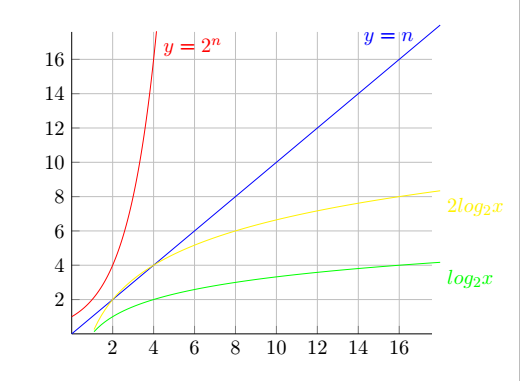
\includegraphics[scale=0.5]{funkcje.PNG}
\textit{ryc.1 - wykres dla funkcji $y=x$(czerwona), $y=x^2$(czarna - rosnąca szybciej), $y=log2(x)$(niebieska), $y=2^x$(zielona), $y=2log2(x)$(czarna - rosnąca wolniej), wygenerowany dzięki stronie: https://www.desmos.com/calculator}
\subsubsection{Najgorszy przypadek}
Istnieje też druga strona medalu i przypadek najgorszy $\theta(n^2)$
\section{Implementacja w Python}
\subsection{Quicksort}
\begin{Verbatim}
def quick_sort(lst, start, stop, fun):
    if start < stop:
        border = fun(lst, start, stop)
        quick_sort(lst, start, border - 1, fun)
        quick_sort(lst, border + 1, stop, fun)
\end{Verbatim}
\subsection{Partition}
\begin{Verbatim}
def partition(lst, start, stop):
    pivot_index = stop
    pivot_value = lst[pivot_index]
    for i in range(start, stop):
        if lst[i] < pivot_value:
            lst[i], lst[start] = lst[start], lst[i]
            start += 1
    lst[stop], lst[start] = lst[start], lst[stop]
    return start
\end{Verbatim}
\newpage
\subsection{Funkcje wyboru pivota}
\begin{Verbatim}
def partition_last(lst, start, stop):
    lst[stop], lst[stop] = lst[stop], lst[stop]
    return partition(lst, start, stop)

def partition_rand(lst, start, stop):
    rand_pivot = random.randint(start, stop)
    lst[stop], lst[rand_pivot] = lst[rand_pivot], lst[stop]
    return partition(lst, start, stop)

def partition_first(lst, start, stop):
    lst[stop], lst[start] = lst[start], lst[stop]
    return partition(lst, start, stop)

def partition_middle(lst, start, stop):
    med = (len(lst)) // 2
    lst[stop], lst[med] = lst[med], lst[stop]
    return partition(lst, start, stop)
\end{Verbatim}
\section{Testy}
\section{Porównanie z innymi algorytmami sortującymi}
\section{Bibliografia}
\end{document}